%%
%% This is file `sample-sigconf.tex',
%% generated with the docstrip utility.
%%
%% The original source files were:
%%
%% samples.dtx  (with options: `all,proceedings,bibtex,sigconf')
%% 
%% IMPORTANT NOTICE:
%% 
%% For the copyright see the source file.
%% 
%% Any modified versions of this file must be renamed
%% with new filenames distinct from sample-sigconf.tex.
%% 
%% For distribution of the original source see the terms
%% for copying and modification in the file samples.dtx.
%% 
%% This generated file may be distributed as long as the
%% original source files, as listed above, are part of the
%% same distribution. (The sources need not necessarily be
%% in the same archive or directory.)
%%
%%
%% Commands for TeXCount
%TC:macro \cite [option:text,text]
%TC:macro \citep [option:text,text]
%TC:macro \citet [option:text,text]
%TC:envir table 0 1
%TC:envir table* 0 1
%TC:envir tabular [ignore] word
%TC:envir displaymath 0 word
%TC:envir math 0 word
%TC:envir comment 0 0
%%
%% The first command in your LaTeX source must be the \documentclass
%% command.
%%
%% For submission and review of your manuscript please change the
%% command to \documentclass[manuscript, screen, review]{acmart}.
%%
%% When submitting camera ready or to TAPS, please change the command
%% to \documentclass[sigconf]{acmart} or whichever template is required
%% for your publication.
%%
%%
% \documentclass[sigconf]{acmart}
\documentclass[sigconf,review,anonymous,screen]{acmart}
%%
%% \BibTeX command to typeset BibTeX logo in the docs
\AtBeginDocument{%
  \providecommand\BibTeX{{%
    Bib\TeX}}}

%%%%%Sid package information here
\input{math_commands}
\usepackage{float}
\usepackage{graphicx}
\usepackage{comment}
\usepackage{setspace}

\usepackage{placeins}

\usepackage{graphicx}
% \usepackage{subfig}
\usepackage{color}
\usepackage{tcolorbox}
\usepackage{amsthm}
\allowdisplaybreaks
\usepackage{multirow}

\usepackage[bottom]{footmisc}
\usepackage{float}
\usepackage{booktabs}
\usepackage{tabularray}
% \usepackage[table]{xcolor}
% \usepackage{subcaption}

\usepackage{xcolor}
\usepackage{hyperref}

\hypersetup{
    colorlinks=true,
    linkcolor=red,
    citecolor=blue,
    urlcolor=blue
}



%\usepackage[table,xcdraw]{xcolor}

\usepackage{tikz}
\usetikzlibrary{trees}
\usepackage{forest}
\usepackage{wrapfig}

% \usepackage{tikz}
\usepackage{adjustbox}
\usetikzlibrary{arrows.meta,positioning,calc}

% ---- compatibility: allow legacy \subfigure{...} with subfig ----
\makeatletter
\@ifundefined{subfigure}{%
  \newcommand{\subfigure}[2][]{\subfloat[#1]{#2}}%
}{}
\makeatother

\usepackage{siunitx}
\sisetup{group-separator={,}, group-minimum-digits=4}


\usepackage{caption}
% \usepackage{subfig}
% \usepackage{subcaption}
\usepackage{colortbl}

\usepackage{graphicx}
% \usepackage{subfigure} %original
\usepackage{subfig} %added sid:
%\captionsetup[subfigure]{list=off}
%\captionsetup[subfigure]{labelformat=empty}
\usepackage{booktabs} % for professional tables


% Attempt to make hyperref and algorithmic work together better:
\newcommand{\theHalgorithm}{\arabic{algorithm}}


\usepackage{xcolor}

\makeatletter
\newcommand{\MODDIV}[1]{%
  \vspace{-0.35\baselineskip}% pull up (reduce the gap above)
  \item[]\makebox[\linewidth][l]{%
    \rule{0.5\linewidth}{0.3pt}\hfill\scriptsize\textbf{#1}%
  }%
  \vspace{-0.55\baselineskip}% pull up next line (reduce the gap below)
}
\makeatother


% \usepackage{booktabs}
\usepackage{pifont}
% \usepackage{amssymb}
% \usepackage{graphicx}
% \usepackage{xcolor}
\usepackage{colortbl}

\usepackage{tikz}
\usetikzlibrary{matrix}

\newcommand{\cmark}{\ding{51}}
\newcommand{\xmark}{\ding{55}}

% \usepackage{tikz}
\usetikzlibrary{arrows.meta, positioning, calc, fit, backgrounds}
\usetikzlibrary{matrix,decorations.pathreplacing}

% %begin-sid
% \newtheorem{assumption}{Assumption}[section]
% % \usepackage{algorithmic}
% % \usepackage{algorithm}
% \usepackage{algorithm}
% \usepackage{multirow}
% \usepackage[linesnumbered,ruled,vlined,algo2e]{algorithm2e}
% \usepackage[inline]{enumitem}

%begin-sid
\newtheorem{assumption}{Assumption}[section]
\usepackage{multirow}
\usepackage[inline]{enumitem}
\usepackage[linesnumbered,ruled,vlined]{algorithm2e}

\SetAlFnt{\small}
\SetAlCapFnt{\small}
\SetAlCapNameFnt{\small}
\SetKwInput{KwIn}{Input}
\SetKwInput{KwOut}{Output}
\SetKwComment{Comment}{/* }{ */}
\DontPrintSemicolon

%for cref
\usepackage[capitalise]{cleveref}

\newcommand{\changes}[1]{{\leavevmode\color{black}#1}}
% \newcommand{\changes}[1]{{\leavevmode\color{blue}#1}}

\newcommand{\payAttention}[3]{\textcolor{#1}{{{#2}: {#3}}}}
% \renewcommand{\payAttention}[3]{}
% \newcommand{\todo}[1]{\payAttention{red}{TODO}{#1}}

\newcommand{\redsays}[2]{\payAttention{red}{#1 Says}{#2}}
\newcommand{\purplesays}[2]{\payAttention{purple}{#1}{#2}}
\newcommand{\naheed}[1]{{\redsays{Naheed}{#1}}}

\newcommand{\xSays}[2]{\payAttention{blue}{#1 Says}{#2}}
\newcommand{\alex}[1]{{\xSays{Alex}{#1}}}
\newcommand{\sid}[1]{\purplesays{Sid}{#1}}
\newcommand{\mahantesh}[1]{\xSays{Mahantesh}{#1}}
\newcommand{\edoardo}[1]{\xSays{Edoardo}{#1}}
\newcommand{\smf}[1]{\xSays{Ferdous}{#1}}
\newcommand{\rounak}[1]{\xSays{Rounak}{#1}}
\newcommand{\erdal}[1]{\xSays{Erdal}{#1}}

\newcommand{\diffgnn}{\texttt{Diff-GNN}\xspace}
\newcommand{\mlp}{\texttt{MLP}\xspace}
\newcommand{\gnn}{\texttt{GNN}\xspace}
\newcommand{\gcn}{\texttt{GCN}\xspace}
% \newcommand{\sigmoid}{\texttt{Sigmoid}\xspace}
% \newcommand{\softmax}{\texttt{Softmax}\xspace}
\newcommand{\relu}{\texttt{ReLU}\xspace}
% \newcommand{\mlp}{\texttt{MLP}\xspace}


%% Rights management information.  This information is sent to you
%% when you complete the rights form.  These commands have SAMPLE
%% values in them; it is your responsibility as an author to replace
%% the commands and values with those provided to you when you
%% complete the rights form.

% Hide ACM reference format and citation info block
\settopmatter{printacmref=false}

% Remove copyright footer
\renewcommand\footnotetextcopyrightpermission[1]{}

% Remove running headers
\pagestyle{plain}

% \setcopyright{acmlicensed}
% \copyrightyear{2018}
% \acmYear{2018}
% \acmDOI{XXXXXXX.XXXXXXX}
% %% These commands are for a PROCEEDINGS abstract or paper.
% \acmConference[Conference acronym 'XX]{Make sure to enter the correct
%   conference title from your rights confirmation email}{June 03--05,
%   2018}{Woodstock, NY}
% %%
% %%  Uncomment \acmBooktitle if the title of the proceedings is different
% %%  from ``Proceedings of ...''!
% %%
% %%\acmBooktitle{Woodstock '18: ACM Symposium on Neural Gaze Detection,
% %%  June 03--05, 2018, Woodstock, NY}
% \acmISBN{978-1-4503-XXXX-X/2018/06}


%%
%% Submission ID.
%% Use this when submitting an article to a sponsored event. You'll
%% receive a unique submission ID from the organizers
%% of the event, and this ID should be used as the parameter to this command.
%%\acmSubmissionID{123-A56-BU3}

%%
%% For managing citations, it is recommended to use bibliography
%% files in BibTeX format.
%%
%% You can then either use BibTeX with the ACM-Reference-Format style,
%% or BibLaTeX with the acmnumeric or acmauthoryear sytles, that include
%% support for advanced citation of software artefact from the
%% biblatex-software package, also separately available on CTAN.
%%
%% Look at the sample-*-biblatex.tex files for templates showcasing
%% the biblatex styles.
%%

%%
%% The majority of ACM publications use numbered citations and
%% references.  The command \citestyle{authoryear} switches to the
%% "author year" style.
%%
%% If you are preparing content for an event
%% sponsored by ACM SIGGRAPH, you must use the "author year" style of
%% citations and references.
%% Uncommenting
%% the next command will enable that style.
%%\citestyle{acmauthoryear}


%%
%% end of the preamble, start of the body of the document source.
\begin{document}

%%
%% The "title" command has an optional parameter,
%% allowing the author to define a "short title" to be used in page headers.
\title{\diffgnn: Differentiable Graph Neural Networks for Joint Hardware-Software Partitioning and Scheduling}

%%
%% The "author" command and its associated commands are used to define
%% the authors and their affiliations.
%% Of note is the shared affiliation of the first two authors, and the
%% "authornote" and "authornotemark" commands
%% used to denote shared contribution to the research.
\author{Ben Trovato}
\authornote{Both authors contributed equally to this research.}
\email{trovato@corporation.com}
\orcid{1234-5678-9012}
\author{G.K.M. Tobin}
\authornotemark[1]
\email{webmaster@marysville-ohio.com}
\affiliation{%
  \institution{Institute for Clarity in Documentation}
  \city{Dublin}
  \state{Ohio}
  \country{USA}
}

\author{Lars Th{\o}rv{\"a}ld}
\affiliation{%
  \institution{The Th{\o}rv{\"a}ld Group}
  \city{Hekla}
  \country{Iceland}}
\email{larst@affiliation.org}

\author{Valerie B\'eranger}
\affiliation{%
  \institution{Inria Paris-Rocquencourt}
  \city{Rocquencourt}
  \country{France}
}

\author{Aparna Patel}
\affiliation{%
 \institution{Rajiv Gandhi University}
 \city{Doimukh}
 \state{Arunachal Pradesh}
 \country{India}}

\author{Huifen Chan}
\affiliation{%
  \institution{Tsinghua University}
  \city{Haidian Qu}
  \state{Beijing Shi}
  \country{China}}

\author{Charles Palmer}
\affiliation{%
  \institution{Palmer Research Laboratories}
  \city{San Antonio}
  \state{Texas}
  \country{USA}}
\email{cpalmer@prl.com}

\author{John Smith}
\affiliation{%
  \institution{The Th{\o}rv{\"a}ld Group}
  \city{Hekla}
  \country{Iceland}}
\email{jsmith@affiliation.org}

\author{Julius P. Kumquat}
\affiliation{%
  \institution{The Kumquat Consortium}
  \city{New York}
  \country{USA}}
\email{jpkumquat@consortium.net}

%%
%% By default, the full list of authors will be used in the page
%% headers. Often, this list is too long, and will overlap
%% other information printed in the page headers. This command allows
%% the author to define a more concise list
%% of authors' names for this purpose.
\renewcommand{\shortauthors}{Das et al.}

%%
%% The abstract is a short summary of the work to be presented in the
%% article.
\begin{abstract}
\sid{
Each paper must be no more than 8 pages (including the abstract, figures, and tables),double-columned, 9pt or 10pt font. One page of references is allowed, which does not count towards this 8-page limitation.
}\sid{(placeholder)} 

% Hardware/software (HW/SW) partitioning is an important problem in embedded system co-design, requiring tasks to be assigned to hardware or software under area constraints while minimizing makespan, i.e., the overall execution time from start to finish.
% HW/SW partitioning is NP-hard and tightly coupled with scheduling, since the execution order of tasks directly affects the final makespan.
% %
% Existing approaches, including mixed-integer linear programming (MILP), metaheuristics, and prior graph-based learning methods, either face scalability limitations, lack optimality guarantees, or do not jointly optimize partitioning and execution ordering in a unified differentiable framework, limiting their ability to consistently find high-quality solutions.
% %
% We present \diffgnn, a differentiable graph neural network (GNN) approach for joint HW/SW partitioning and scheduling. The proposed model combines a GNN encoder with a placement head for assignment prediction and an ordering head that learns execution priorities through a differentiable relaxation.
% Unlike prior approaches, \diffgnn embeds task-order learning into the optimization itself, enabling end-to-end learning of both placement and scheduling decisions in a unified manner. We introduce a soft scheduling surrogate that approximates makespan under hardware-area constraints.
% %
% We further incorporate a post-processing and refinement module that converts relaxed predictions into feasible discrete assignments and improves final solution quality. A practical strength of \diffgnn is that it is optimized directly on the given task graph, eliminating the need for a separate corpus of training graphs.
% %
% Across task graphs derived from neural network workloads, \diffgnn achieves lower makespan than metaheuristics and prior GNN-based HW/SW partitioning approaches, while remaining competitive with MILP on small and medium instances. In contrast to MILP, however, \diffgnn remains practical on larger graphs where exact optimization becomes computationally prohibitive. These results show that differentiable joint placement and order learning provide a scalable and effective new direction for HW/SW partitioning.
% Code is available at \url{https://github.com/anonymousauthors001/diff_gnn}
\end{abstract}



%%
%% The code below is generated by the tool at http://dl.acm.org/ccs.cfm.
%% Please copy and paste the code instead of the example below.
%%
% \begin{CCSXML}
% <ccs2012>
%  <concept>
%   <concept_id>00000000.0000000.0000000</concept_id>
%   <concept_desc>Do Not Use This Code, Generate the Correct Terms for Your Paper</concept_desc>
%   <concept_significance>500</concept_significance>
%  </concept>
%  <concept>
%   <concept_id>00000000.00000000.00000000</concept_id>
%   <concept_desc>Do Not Use This Code, Generate the Correct Terms for Your Paper</concept_desc>
%   <concept_significance>300</concept_significance>
%  </concept>
%  <concept>
%   <concept_id>00000000.00000000.00000000</concept_id>
%   <concept_desc>Do Not Use This Code, Generate the Correct Terms for Your Paper</concept_desc>
%   <concept_significance>100</concept_significance>
%  </concept>
%  <concept>
%   <concept_id>00000000.00000000.00000000</concept_id>
%   <concept_desc>Do Not Use This Code, Generate the Correct Terms for Your Paper</concept_desc>
%   <concept_significance>100</concept_significance>
%  </concept>
% </ccs2012>
% \end{CCSXML}

% \ccsdesc[500]{Do Not Use This Code~Generate the Correct Terms for Your Paper}
% \ccsdesc[300]{Do Not Use This Code~Generate the Correct Terms for Your Paper}
% \ccsdesc{Do Not Use This Code~Generate the Correct Terms for Your Paper}
% \ccsdesc[100]{Do Not Use This Code~Generate the Correct Terms for Your Paper}

%%
%% Keywords. The author(s) should pick words that accurately describe
%% the work being presented. Separate the keywords with commas.
% \keywords{Do, Not, Use, This, Code, Put, the, Correct, Terms, for,
%   Your, Paper}
%% A "teaser" image appears between the author and affiliation
%% information and the body of the document, and typically spans the
%% page.
% \begin{teaserfigure}
%   \includegraphics[width=\textwidth]{sampleteaser}
%   \caption{Seattle Mariners at Spring Training, 2010.}
%   \Description{Enjoying the baseball game from the third-base
%   seats. Ichiro Suzuki preparing to bat.}
%   \label{fig:teaser}
% \end{teaserfigure}

% \received{20 February 2007}
% \received[revised]{12 March 2009}
% \received[accepted]{5 June 2009}

%%
%% This command processes the author and affiliation and title
%% information and builds the first part of the formatted document.
\maketitle

\section{Introduction}
\noindent\textbf{Our contributions are as follows:}

\begin{itemize}
    \item We present \diffgnn, a differentiable framework for jointly optimizing HW/SW partitioning and software-task ordering under hardware area constraints.

    \item We introduce a differentiable ordering head based on Sinkhorn relaxation, which enables software execution priorities to be learned jointly with placement decisions.

    \item We develop an order-aware soft scheduling surrogate that captures precedence, communication, and software serialization, enabling end-to-end optimization toward makespan minimization.

    \item We design a discrete inference pipeline with decoding, feasibility repair, and refinement, which produces valid solutions under area constraints and improves robustness to relaxation error.

    \item We evaluate \diffgnn against exact optimization, metaheuristic, and prior learning-based baselines on task graphs derived from neural network workloads, demonstrating competitive solution quality and improved scalability.
\end{itemize}
\section{Related Works}

\begin{itemize}
    \item GCN-based HW/SW partitioning 2021~\citep{zheng2021hardware}
    \item HW/SW partitioning survey 2019~\cite{hou2019survey}, 
    HW/SW partitioning survey 2012~\citep{teich2012hardware} %https://ieeexplore.ieee.org/stamp/stamp.jsp?arnumber=6172642
    \item Arato~\citep{arato2005algorithmic}
    \item Family of exact solutions includes Dynamic Programming (DP)~\citep{}, Integer Linear Programming (ILP)~\citep{}, Branch and Bound (BB)~\citep{}.
    
    \item The common metaheuristics discussed in the literature for HW/SW partitioning are Genetic Algorithms~\citep{}, Simulated Annealing~\citep{}, and Tabu Search (TS)~\citep{}. These works for graph with small number of nodes.

    \item ILP limitation is $\le 400$ nodes task graph~\citep{trindade2016applying}.
    
    Ant colony optimization (ACO)~\citep{}, artificial bees~\citep{}, particle swarm optimization (PSO)~\citep{}, artificial immune algorithm~\citep{}. Due to the complexity of the problem and the limitations of runtime, it is almost impossible for these metaheuristics to achieve global optimization~\citep{hou2019survey}.

    \item Another category of general heuristics is to reduce this HW/SW partitioning problem into another classical NP hard paroblems, such as graph partitioning~\citep{arato2005algorithmic}, or Knapsack problem~\citep{}
    
    
\end{itemize}

The HW/SW partitioning problem can be formalized as a bi-partitioning problem to find the global optimal solution~\citep{han2013efficient}.



\section{Problem Setup}
\label{sec:preliminaries}

We consider a target architecture consisting of a single software processor and multiple hardware (ASIC/FPGA) components. Software tasks execute sequentially on the CPU, while hardware tasks without dependencies can execute in parallel. Communication between tasks assigned to different platforms incurs an interconnect transfer cost, modeled as an edge-dependent communication delay. Assignments must satisfy a global hardware area constraint. The goal of HW/SW partitioning is to assign tasks to hardware or software to minimize end-to-end execution time under this constraint.

\subsection{Problem formulation}
We are given a task graph $\gG(\gV,\gE)$ with $|\gV|=n$ nodes and $|\gE|=m$ edges, modeled as a directed acyclic graph (DAG), as shown in Figure~\ref{fig:sampletaskgraph}. Each node $i \in \gV$ has software and hardware execution costs $t_i^{sw}$ and $t_i^{hw}$, respectively, and requires hardware area $A_i$ if assigned to hardware. Each edge $(j,i)\in\gE$ represents a precedence dependency from task $j$ to task $i$, with communication cost $C_{ji}$ incurred when the two endpoint tasks are assigned to different platforms.

\begin{figure}[!htbp]
\centering
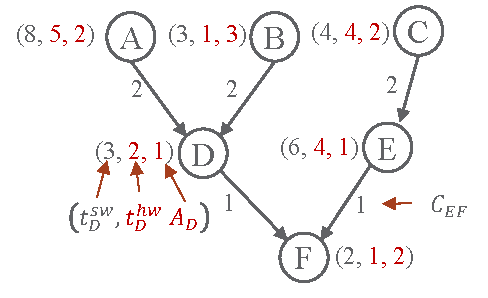
\includegraphics[width=0.5\linewidth]{Figures/introduction/taskgraph.pdf}
\caption{Sample task graph for HW/SW partitioning. Each node shows its software cost, hardware cost, and required hardware area. Directed edges indicate task dependencies, and edge labels represent communication cost when connected tasks are assigned to different types.}
\label{fig:sampletaskgraph}
\end{figure}

We represent a discrete HW/SW partition using a binary vector $\vp \in \{0,1\}^n$, where $p_i=1$ denotes hardware assignment and $p_i=0$ denotes software assignment for node $i$. Since software tasks share a single processor, the final makespan also depends on their execution order. Let $\pi^{sw}$ denote a valid rank-based order over software tasks, where
\begin{equation}
\pi_i^{sw} < \pi_j^{sw}
\;\Longrightarrow\;
i \prec_{\pi^{sw}} j,
\end{equation}
meaning that task $i$ is scheduled before task $j$ on the software processor.
Given an assignment $\vp$ and software order $\pi^{sw}$, let $(\vs, \vf)\gets \mathrm{Sched}(\vp,\pi^{sw})$ denote the induced schedule that returns the corresponding start-time and finish-time vectors $\vs$ and $\vf$. The makespan under assignment $\vp$ and software order $\pi^{sw}$ is defined as
\begin{equation}
M(\vp,\pi^{sw}) = \max_{i\in\gV} f_i.
\label{eq:true_makespan}
\end{equation}

Our goal is to minimize makespan under the hardware area budget:
\begin{align}
\min_{\vp \in \{0,1\}^n,\;\pi^{sw}} \quad
& M(\vp,\pi^{sw}) = \max_{i\in\gV} f_i
\label{eq:true_obj}\\
\text{s.t.}\quad
& (\vs,\vf)=\mathrm{Sched}(\vp,\pi^{sw}),
\label{eq:true_sched}\\
& \sum_{i\in\gV} p_i A_i \le A_{\max},
\label{eq:true_area}\\
& f_i = s_i + \underbrace{p_i t_i^{hw} + (1-p_i)t_i^{sw}}_{\mathrm{Execution}},
\qquad \forall i\in\gV,
\label{eq:true_finish}\\
& s_i \ge f_j + \underbrace{\mathbb{I}[p_j \neq p_i]\, C_{ji}}_{\mathrm{Communication}},
\qquad \forall (j,i)\in\gE,
\label{eq:true_pred}\\
& s_j \ge f_i,
\qquad \forall i,j\in\gV: p_i=p_j=0
\text{ and } i \prec_{\pi^{sw}} j,
\label{eq:true_sw_serial}\\
& s_i \ge 0,
\qquad \forall i\in\gV.
\label{eq:true_nonneg}
\end{align}

Equation~\eqref{eq:true_finish} defines the finish time of each task under the chosen assignment. Equation~\eqref{eq:true_pred} enforces precedence constraints together with inter-platform communication delay. Equation~\eqref{eq:true_sw_serial} enforces sequential execution of software-assigned tasks according to the order $\pi^{sw}$. Hardware-assigned tasks may execute in parallel as long as the precedence constraints are satisfied.


\subsection{Differentiable Relaxation of the Discrete Problem}

Directly optimizing Equations~\eqref{eq:true_obj}--\eqref{eq:true_nonneg} is difficult because both the placement vector $\vp \in \{0,1\}^n$ and the software order $\pi^{sw}$ are discrete. In \diffgnn, we therefore relax the binary assignment vector $\vp$ to a continuous vector $\tilde{\vp}\in[0,1]^n$, where $\tilde{p}_i$ denotes the confidence of assigning task $i$ to hardware. To approximate the discrete software order $\pi^{sw}$, the GNN also predicts a continuous software-priority vector $\tilde{\vpi}^{sw}\in[-1,1]^n$. These values encode relative precedence among software tasks: if $\tilde{\pi}_i^{sw} > \tilde{\pi}_j^{sw}$, then the relaxed model prefers $i \prec j$. Sorting $\tilde{\vpi}^{sw}$ induces a discrete rank-based order that approximates $\pi^{sw}$.

Under this relaxation, the execution-time expression in Equation~\eqref{eq:true_finish} becomes
\begin{equation}
\tilde{t}_i(\tilde{\vp})
=
\tilde{p}_i t_i^{hw} + (1-\tilde{p}_i)t_i^{sw},
\label{eq:soft_exec_i}
\end{equation}
and the communication term in Equation~\eqref{eq:true_pred} is approximated by
\begin{equation}
\tilde{c}_{ji}(\tilde{\vp})
=
|\tilde{p}_j-\tilde{p}_i|\, C_{ji}.
\label{eq:soft_comm_ji}
\end{equation}

Similarly, instead of the discrete schedule $(\vs,\vf)=\mathrm{Sched}(\vp,\pi^{sw})$, we define a differentiable surrogate scheduler
\begin{equation}
(\tilde{\vs},\tilde{\vf})
=
\widetilde{\mathrm{Sched}}(\tilde{\vp},\tilde{\vpi}^{sw}),
\label{eq:soft_sched}
\end{equation}
which approximates the precedence, communication, and software-serialization constraints in Equations~\eqref{eq:true_pred}--\eqref{eq:true_sw_serial}.

The max operator appearing in the makespan and readiness computations is not differentiable. We therefore replace it with the smooth maximum operator
\begin{equation}
\mathrm{SMax}_{\beta}(\{a_k\})
=
\frac{1}{\beta}\log\sum_k e^{\beta a_k},
\label{eq:smax_beta}
\end{equation}
where $\beta>0$ controls the sharpness of the approximation. As $\beta$ increases, $\mathrm{SMax}_{\beta}$ approaches the standard max operator.

\paragraph{\textbf{Precedence relation of Equation~\eqref{eq:true_pred}}}
Let $\Pred(i)$ denote the set of predecessors of node $i$. The relaxed DAG-readiness term is defined as
\begin{equation}
s_i^{dag}
=
\begin{cases}
0, & \Pred(i)=\emptyset,\\[4pt]
\mathrm{SMax}_{\beta}
\Big(
\{\, \tilde{f}_j + \tilde{c}_{ji}(\tilde{\vp}) \mid j \in \Pred(i)\,\}
\Big), & \text{otherwise},
\end{cases}
\label{eq:soft_rdag}
\end{equation}
which approximates the earliest time at which task $i$ becomes ready from the precedence perspective of Equation~\eqref{eq:true_pred}.

\paragraph{\textbf{SW relation of Equation~\eqref{eq:true_sw_serial}}}
To capture serialization on the software processor in Equation~\eqref{eq:true_sw_serial}, we define the relaxed software-readiness term as
\begin{equation}
s_i^{sw}
=
\mathrm{SMax}_{\beta}
\Big(
\{\, \tilde{f}_j + \phi_{sw}(\tilde{\pi}_j^{sw}, \tilde{\pi}_i^{sw}) \mid j \neq i\,\}
\Big),
\label{eq:soft_rsw}
\end{equation}
where $\phi_{sw}(\cdot)$ is a differentiable ordering function that maps the relative priority difference between tasks $j$ and $i$ to a soft serialization penalty. Intuitively, if $\tilde{\pi}_j^{sw}$ indicates that task $j$ should execute before task $i$, then the contribution of $\tilde{f}_j$ to $s_i^{sw}$ becomes stronger. The explicit construction of $\phi_{sw}$ is introduced later in the proposed method.

\paragraph{\textbf{Soft makespan of Equation~\eqref{eq:true_makespan}}}
The relaxed start and finish times are then
\begin{equation}
\tilde{s}_i
=
\mathrm{SMax}_{\beta}\big(\{s_i^{dag},\, s_i^{sw}\}\big),
\label{eq:soft_start}
\end{equation}
\begin{equation}
\tilde{f}_i
=
\tilde{s}_i + \tilde{t}_i(\tilde{\vp}),
\label{eq:soft_finish}
\end{equation}
which mirror the discrete scheduling relations in Equations~\eqref{eq:true_finish}--\eqref{eq:true_sw_serial}.

Let $\Sink(\gG)$ denote the set of sink nodes in $\gG$. The differentiable surrogate makespan is defined as
\begin{equation}
\widetilde{M}(\tilde{\vp},\tilde{\vpi}^{sw})
=
\mathrm{SMax}_{\beta}\big(\{\, \tilde{f}_i \mid i \in \Sink(\gG)\,\}\big).
\label{eq:soft_makespan_symbol}
\end{equation}

\paragraph{\textbf{Area of Equation~\eqref{eq:true_area}}}
To encourage feasibility under the hardware budget in Equation~\eqref{eq:true_area}, we use the differentiable area penalty
\begin{equation}
\mathcal{L}_{\mathrm{area}}(\tilde{\vp})
=
\left[
\max\left(
0,\;
\sum_{i\in\gV}\tilde{p}_i A_i - A_{\max}
\right)
\right]^2.
\label{eq:l_area}
\end{equation}

\paragraph{\textbf{Relaxed objective}}
The relaxed objective optimized by \diffgnn is therefore
\begin{equation}
\mathcal{L}_{\mathrm{relax}}(\tilde{\vp},\tilde{\vpi}^{sw})
=
\widetilde{M}(\tilde{\vp},\tilde{\vpi}^{sw})
+
\lambda_a \mathcal{L}_{\mathrm{area}}(\tilde{\vp}).
\label{eq:relaxed_obj}
\end{equation}

Thus, while the original problem minimizes makespan over the discrete placement vector $\vp$ and software order $\pi^{sw}$, \diffgnn is trained by minimizing the continuous surrogate in Equation~\eqref{eq:relaxed_obj}. Auxiliary execution, communication, and regularization terms used in practice are introduced later in the proposed method.

\begin{figure*}[!htbp]
\centering
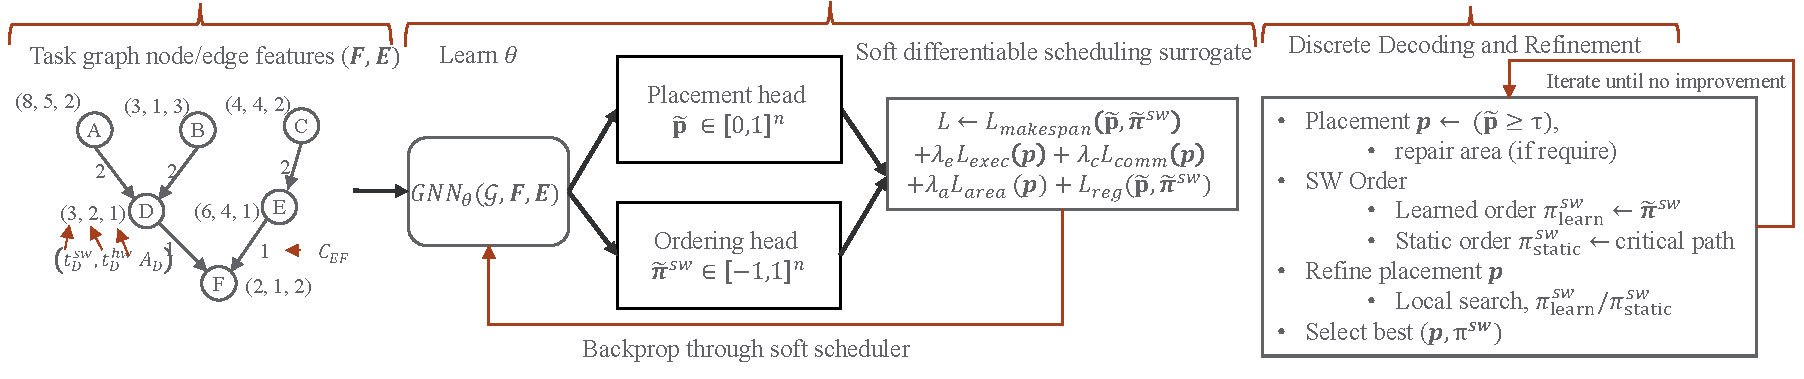
\includegraphics[width=1.0\linewidth]{Figures/methods/GNN_placement_order.pdf}
\caption{\sid{placeholder} Overview of \diffgnn for joint HW/SW partitioning and scheduling. A GNN encoder maps task graph features to the relaxed placement vector $\tilde{\vp}$ and relaxed software-priority vector $\tilde{\vpi}^{sw}$. A differentiable scheduling surrogate enables end-to-end optimization of makespan under constraints. At inference, solutions are discretized, repaired for feasibility, optionally refined, and evaluated using both the learned software order and a heuristic static-priority order; the better schedule is retained.}
\label{fig:diff_gnn_architecture}
\end{figure*}

\section{Proposed Method: \diffgnn}
\label{sec:method}

Building on the relaxed formulation in Section~\ref{sec:preliminaries}, we propose \diffgnn, a differentiable graph neural framework for jointly optimizing HW/SW partitioning and scheduling. Rather than directly searching over the discrete placement vector $\vp \in \{0,1\}^n$ and software order $\pi^{sw}$, \diffgnn learns a relaxed hardware-assignment vector $\tilde{\vp}\in[0,1]^n$ together with a relaxed software-priority vector $\tilde{\vpi}^{sw}\in[-1,1]^n$, and optimizes the relaxed objective in Equation~\eqref{eq:relaxed_obj} end-to-end using gradient-based learning.

Figure~\ref{fig:diff_gnn_architecture} illustrates the overall pipeline. Given a task graph $\gG(\gV,\gE)$, we first construct node and edge features, and a GNN encoder computes node embeddings that are then consumed by two prediction heads: (i) a \emph{placement head} that predicts relaxed hardware-assignment probabilities, and (ii) an \emph{ordering head} that predicts relaxed software priorities. These outputs are passed to an order-aware differentiable scheduler that approximates the makespan while accounting for both precedence constraints and software serialization. During inference, the relaxed solution is discretized, repaired if necessary to satisfy the area constraint, optionally refined, and finally evaluated using a discrete scheduler under two candidate software orders: the learned order induced by $\tilde{\vpi}^{sw}$ and a heuristic static-priority order. The better schedule is selected as the final output.


\subsection{Input Feature Preparation}

\paragraph{\textbf{Node features.}}
Each node $i \in \gV$ is associated with a feature vector capturing execution cost, resource usage, and structural properties:
\begin{equation}
\vf_i^{\mathrm{raw}} =
\left[
t_i^{sw},\;
t_i^{hw},\;
A_i,\;
d_i,\;
\frac{t_i^{hw}}{t_i^{sw}+\epsilon},\;
t_i^{sw}-t_i^{hw},\;
\frac{t_i^{sw}-t_i^{hw}}{\max(A_i,\epsilon)}
\right]
\in \mathbb{R}^7.
\end{equation}

Stacking all node features yields
\begin{equation}
\mF^{\mathrm{raw}} =
\begin{bmatrix}
(\vf_1^{\mathrm{raw}})^\top\\
\vdots\\
(\vf_n^{\mathrm{raw}})^\top
\end{bmatrix}
\in \mathbb{R}^{n\times 7}.
\end{equation}

We normalize features across nodes using column-wise z-score normalization:
\begin{equation}
\tilde{\mF} = \mathrm{Norm}(\mF^{\mathrm{raw}}).
\end{equation}

To incorporate the global hardware-area constraint, we append a constant feature:
\begin{equation}
\mF=
\begin{bmatrix}
\tilde{\mF} & \rho_A \mathbf{1}
\end{bmatrix}
\in\mathbb{R}^{n\times 8},
\end{equation}
where $\mathbf{1}\in\mathbb{R}^n$ is the all-ones vector.

\paragraph{\textbf{Edge features.}}
For each directed edge $(j,i)\in\gE$, we define an edge feature vector:
\begin{equation}
\ve_{ji}^{\mathrm{raw}} =
\left[
C_{ji},\;
|g_j-g_i|,\;
|ga_j-ga_i|
\right]
\in \mathbb{R}_{\ge 0}^3.
\end{equation}

Stacking all edges yields
\begin{equation}
\mE^{\mathrm{raw}} \in \mathbb{R}^{|\gE|\times 3}.
\end{equation}

We normalize edge features using column-wise max scaling:
\begin{equation}
\mE = \mathrm{Norm}_\infty(\mE^{\mathrm{raw}}),
\end{equation}
where $\mathrm{Norm}_\infty(\cdot)$ denotes feature-wise normalization by the maximum value.

\subsection{GNN Module}

\paragraph{\textbf{Message passing.}}
Let $\vh_i^{(0)}=\mF_{i,:}$ denote the initial node embedding. We use a message-passing GNN with $L$ layers:
\begin{equation}
\vh_i^{(\ell+1)}=
\phi^{(\ell)}\!\left(
\vh_i^{(\ell)},
\operatorname*{AGG}_{j:(j,i)\in\gE}
\psi^{(\ell)}\!\left(
\vh_i^{(\ell)},\;
\vh_j^{(\ell)},\;
\ve_{ji}
\right)
\right),
\end{equation}
for $\ell=0,\dots,L-1$, where $\phi^{(\ell)}$ and $\psi^{(\ell)}$ are learnable functions and $\operatorname*{AGG}$ is a permutation-invariant aggregation operator.

As a concrete instantiation, we use weighted mean aggregation:
\begin{align*}
\operatorname*{AGG}_{j:(j,i)\in\gE}
\psi^{(\ell)}\!\left(
\vh_i^{(\ell)},\;
\vh_j^{(\ell)},\;
\ve_{ji}
\right)
&=\frac{1}{\alpha}\sum_{j\in\gN(i)}\alpha_{\phi}(j,i)\,\mathbf{W}^{(\ell)}\vh_j^{(\ell)},\\
\alpha &= \sum_{j\in\gN(i)} \alpha_{\phi}(j,i)+\epsilon,
\end{align*}
where $\gN(i)$ denotes the set of incoming neighbors of node $i$, $\mathbf{W}^{(\ell)}$ is a learnable linear transformation, and $\alpha_{\phi}(j,i)\ge 0$ is a learnable edge weight derived from $\ve_{ji}$. We compute
\begin{equation}
\alpha_{\phi}(j,i)=\sigma\!\left(f_{\phi}(\ve_{ji})\right),
\end{equation}
where $f_{\phi}$ is an MLP and $\sigma(\cdot)$ is the sigmoid function.

\paragraph{\textbf{Placement head.}}
From the final embedding $\vh_i^{(L)}$, we predict relaxed hardware-assignment probabilities:
\begin{equation}
\tilde{p}_i = \sigma\!\left(\mathrm{MLP}_{\mathrm{place}}(\vh_i^{(L)})\right),
\end{equation}
where $\sigma(\cdot)$ denotes the sigmoid function, ensuring $\tilde{p}_i\in(0,1)$. Stacking all node-wise predictions gives
\begin{equation}
\tilde{\vp} = [\tilde{p}_1,\dots,\tilde{p}_n]^\top .
\end{equation}

\paragraph{\textbf{Ordering head.}}
To model software execution order, we compute bounded relaxed software-priority values:
\begin{equation}
\tilde{\pi}_i^{sw} = \tanh\!\left(\mathrm{MLP}_{\mathrm{order}}(\vh_i^{(L)})\right),
\end{equation}
so that $\tilde{\pi}_i^{sw}\in(-1,1)$. Stacking them yields
\begin{equation}
\tilde{\vpi}^{sw} = [\tilde{\pi}_1^{sw},\dots,\tilde{\pi}_n^{sw}]^\top \in \mathbb{R}^n.
\end{equation}


\subsection{Differentiable Soft Scheduler}

We now instantiate the relaxed makespan term $\widetilde{M}(\tilde{\vp},\tilde{\vpi}^{sw})$ from Section~\ref{sec:preliminaries}. The scheduler takes as input the relaxed placement vector $\tilde{\vp}$ and the relaxed software-priority vector $\tilde{\vpi}^{sw}$, and produces approximate start and finish times for all tasks.

The most important intermediate quantity is the effective software-order matrix $R^{sw}$. Figure~\ref{fig:soft_scheduler_walkthrough} illustrates its construction on a 6-node example. Read the figure from left to right:
\[
\tilde{\vpi}^{sw}
\;\rightarrow\;
\mP^{sw}
\;\rightarrow\;
\tilde{\vr}
\;\rightarrow\;
\mB^{sw}
\;\rightarrow\;
\mR^{sw}
\;\rightarrow\;
\widetilde{M}(\tilde{\vp},\tilde{\vpi}^{sw}).
\]

\begin{figure*}[t]
\centering
\setlength{\tabcolsep}{2.2pt}
\renewcommand{\arraystretch}{1.0}
\begin{adjustbox}{width=\textwidth,center}
\begin{tikzpicture}[
    >=Latex,
    font=\scriptsize,
    box/.style={draw=black!55, rounded corners=1pt, fill=gray!5, inner sep=2.2pt, align=center},
    arr/.style={-{Latex[length=1.8mm]}, very thick, draw=orange!85!black}
]

% =========================================================
% 1) GRAPH + INPUTS
% =========================================================
\node[anchor=north west] (graphbox) at (0,0) {%
\begin{minipage}{0.20\textwidth}
\centering
\begin{tikzpicture}[scale=0.68, every node/.style={font=\scriptsize}]
\node[circle,draw,fill=orange!85!yellow,inner sep=1.6pt,label=above:{A $(8,5,2)$}] (A) at (0,1.8) {};
\node[circle,draw,fill=orange!85!yellow,inner sep=1.6pt,label=above:{B $(3,1,3)$}] (B) at (1.9,1.8) {};
\node[circle,draw,fill=orange!85!yellow,inner sep=1.6pt,label=above:{C $(4,4,2)$}] (C) at (3.8,1.8) {};
\node[circle,draw,fill=black!90,inner sep=1.6pt,label=left:{D $(3,2,1)$}] (D) at (0.95,0.7) {};
\node[circle,draw,fill=black!90,inner sep=1.6pt,label=right:{E $(6,4,1)$}] (E) at (2.85,0.7) {};
\node[circle,draw,fill=black!90,inner sep=1.6pt,label=below:{F $(2,1,2)$}] (F) at (1.90,-0.35) {};
\draw[->,thin] (A)-- node[left] {\scriptsize 2} (D);
\draw[->,thin] (B)-- node[left] {\scriptsize 2} (D);
\draw[->,thin] (C)-- node[right] {\scriptsize 2} (E);
\draw[->,thin] (D)-- node[below] {\scriptsize 0} (F);
\draw[->,thin] (E)-- node[below] {\scriptsize 0} (F);
\end{tikzpicture}

\vspace{0.8mm}
$\tilde{\vp}=[0.05,0.05,0.05,0.95,0.95,0.95]^\top$

$\tilde{\vpi}^{sw}=[0.00,-1.00,1.00,-0.50,-0.75,-0.25]^\top$

Induced SW order: $C \prec A \prec B$
\end{minipage}
};

% =========================================================
% 2) ORDER VECTOR
% =========================================================
\node[box, anchor=north west] (qtab) at (4.25,0) {%
\begin{tabular}{c|c}
Task & $\tilde{\pi}^{sw}$\\\hline
A & \textcolor{red}{0.00}\\
B & \textcolor{red}{-1.00}\\
C & \textcolor{red}{1.00}\\
D & -0.50\\
E & -0.75\\
F & -0.25
\end{tabular}
};

% =========================================================
% 3) SINKHORN MATRIX
% =========================================================
\node[box, anchor=north west] (pmat) at (6.15,0) {%
\begin{tabular}{c|cccccc}
$u_a$ & A & B & C & D & E & F\\\hline
1.0  & 0.181 & 0.002 & \textcolor{red}{0.695} & 0.029 & 0.008 & 0.084\\
0.6  & \textcolor{red}{0.332} & 0.015 & 0.257 & 0.120 & 0.047 & 0.229\\
0.2  & 0.271 & 0.060 & 0.043 & 0.218 & 0.128 & 0.280\\
-0.2 & 0.143 & 0.155 & 0.005 & 0.255 & 0.224 & 0.219\\
-0.6 & 0.056 & 0.302 & 0.000 & 0.223 & 0.291 & 0.128\\
-1.0 & 0.017 & \textcolor{red}{0.467} & 0.000 & 0.155 & 0.302 & 0.060
\end{tabular}
};

\node[font=\scriptsize] at ($(pmat.south)+(0,-0.28)$)
{$L_{ai}=-(\tilde{\pi}^{sw}_i-u_a)^2/\tau_o,\quad \mP^{sw}=\mathrm{Sinkhorn}(L)$};

% =========================================================
% 4) RANK TABLE
% =========================================================
\node[box, anchor=north west] (rtab) at (11.10,0) {%
\begin{tabular}{c|c}
Task & $\tilde r_i$\\\hline
A & \textcolor{red}{1.613}\\
B & \textcolor{red}{4.141}\\
C & \textcolor{red}{0.357}\\
D & 2.986\\
E & 3.649\\
F & 2.258
\end{tabular}
};

\node[font=\scriptsize] at ($(rtab.south)+(0,-0.28)$)
{$\tilde r_i=\sum_{a=0}^{n-1} a\,\mP^{sw}_{ai}$};

% =========================================================
% 5) COMBINED GATE + BEFORE BOX
% =========================================================
\node[box, anchor=north west] (gbbox) at (13.00,0) {%
\begin{minipage}{0.23\textwidth}
\centering
$\displaystyle
G^{sw}=(1-\tilde{\vp})(1-\tilde{\vp})^\top=
\begin{bmatrix}
0.903\,\mathbf{1}_{3\times3} & 0.048\,\mathbf{1}_{3\times3}\\
0.048\,\mathbf{1}_{3\times3} & 0.003\,\mathbf{1}_{3\times3}
\end{bmatrix}
$

\vspace{0.8mm}
\begin{tabular}{c|cccccc}
 & A & B & C & D & E & F\\\hline
A & 0     & 0.999 & 0.027 & 0.981 & 0.997 & 0.863\\
B & 0.001 & 0     & 0     & 0.036 & 0.197 & 0.005\\
C & \textcolor{red}{0.973} & \textcolor{red}{1.000} & 0 & 0.999 & 1.000 & 0.996\\
D & 0.019 & 0.964 & 0.001 & 0 & 0.869 & 0.111\\
E & 0.003 & 0.803 & 0 & 0.131 & 0 & 0.018\\
F & 0.137 & 0.995 & 0.004 & 0.889 & 0.982 & 0
\end{tabular}

\vspace{0.6mm}
$\displaystyle B^{sw}_{ji}=\sigma\!\left(\frac{\tilde r_i-\tilde r_j}{\tau_r}\right)$
\end{minipage}
};

% =========================================================
% 6) FINAL RESOURCE MATRIX
% =========================================================
\node[box, anchor=north west] (rmat) at (18.00,0) {%
\begin{tabular}{c|cccccc}
 & A & B & C & D & E & F\\\hline
A & 0     & 0.902 & \textcolor{red}{0.024} & 0.047 & 0.047 & 0.041\\
B & 0.001 & 0     & 0     & 0.002 & 0.009 & 0\\
C & \textcolor{red}{0.878} & \textcolor{red}{0.902} & 0 & 0.047 & 0.047 & 0.047\\
D & 0.001 & 0.046 & 0 & 0 & 0.002 & 0\\
E & 0 & 0.038 & 0 & 0 & 0 & 0\\
F & 0.006 & 0.047 & 0 & 0.002 & 0.002 & 0
\end{tabular}
};

\node[font=\scriptsize] at ($(rmat.south)+(0,-0.28)$)
{$R^{sw}=B^{sw}\odot G^{sw}$};

\node[font=\scriptsize] at ($(rmat.south)+(0,-0.68)$)
{Key entries: $R^{sw}_{CA}=0.878,\;R^{sw}_{CB}=0.902,\;R^{sw}_{AB}=0.902$};

% =========================================================
% 7) MAKESPAN BOX
% =========================================================
\node[anchor=north west] (mspan) at (22.65,0) {%
\begin{minipage}{0.27\textwidth}
\centering
\textbf{From $R^{sw}$ to relaxed makespan}

\vspace{0.8mm}
Using the induced order $C \prec A \prec B$:
\[
\tilde f_C=4.00,\quad \tilde f_A=11.85,\quad \tilde f_B=14.75
\]
\[
\tilde s_D=16.55,\ \tilde f_D=18.60,\qquad
\tilde s_E=5.80,\ \tilde f_E=9.90
\]
\[
\tilde s_F=18.60,\qquad \tilde f_F=19.65
\]
\[
\widetilde{M}(\tilde{\vp},\tilde{\vpi}^{sw})
=
\mathrm{SMax}_{\beta}\!\big(\{\tilde f_i:i\in\Sink(\gG)\}\big)
\approx 19.65
\]

Alternative order $A \prec B \prec C$:
\[
\tilde f_F\approx 21.70
\]
Hence the learned ordering reduces the relaxed makespan.
\end{minipage}
};

% =========================================================
% ARROWS
% =========================================================
\draw[arr] (graphbox.east) -- (qtab.west);
\draw[arr] (qtab.east) -- (pmat.west);
\draw[arr] (pmat.east) -- (rtab.west);
\draw[arr] (rtab.east) -- (gbbox.west);
\draw[arr] (gbbox.east) -- (rmat.west);
\draw[arr] (rmat.east) -- (mspan.west);

\end{tikzpicture}
\end{adjustbox}
\caption{Numerical walk-through of the soft scheduler on a 6-node example. The example graph and relaxed inputs are followed by the ordering vector, Sinkhorn soft permutation matrix, expected ranks, gated rank-based precedence structure, effective software-order matrix $R^{sw}$, and the resulting relaxed makespan computation. The highlighted entries show that the example strongly favors the software order $C \prec A \prec B$.}
\label{fig:soft_scheduler_walkthrough}
\end{figure*}
First, the ordering head predicts relaxed software priorities $\tilde{\vpi}^{sw}$. These values are converted into a soft permutation matrix $\mP^{sw}$ using Sinkhorn normalization; $\mP^{sw}$ is then mapped to expected ranks $\tilde r_i$; the ranks are converted into a pairwise before matrix $\mB^{sw}$; and finally $\mB^{sw}$ is gated by the software co-assignment matrix so that ordering affects only tasks that are likely mapped to software. The same figure then shows how the resulting order propagates to the relaxed start and finish times and, ultimately, to the relaxed makespan.

\paragraph{\textbf{From relaxed software priorities to the effective software-order matrix.}}
The ordering head outputs
\begin{equation}
\tilde{\vpi}^{sw}=[\tilde{\pi}_1^{sw},\ldots,\tilde{\pi}_n^{sw}]^\top.
\end{equation}
We first construct a score-to-position compatibility matrix
\begin{equation}
L_{ai}=-\frac{(\tilde{\pi}_i^{sw}-u_a)^2}{\tau_o},
\qquad
u_a=1-\frac{2a}{n-1},
\quad a=0,\ldots,n-1,
\end{equation}
where $\{u_a\}_{a=0}^{n-1}$ are evenly spaced position anchors and $\tau_o$ controls the sharpness of the relaxation. Applying Sinkhorn normalization gives
\begin{equation}
\mP^{sw}=\mathrm{Sinkhorn}(L)\in[0,1]^{n\times n},
\end{equation}
where $\mP^{sw}_{ai}$ is the soft probability that task $i$ occupies position $a$ in the software order.

Next we compute the expected rank of each task:
\begin{equation}
\tilde r_i=\sum_{a=0}^{n-1} a\,\mP^{sw}_{ai}.
\end{equation}
A smaller $\tilde r_i$ indicates that task $i$ is predicted to execute earlier on software. We then convert these ranks into pairwise precedence scores:
\begin{equation}
B^{sw}_{ji}
=
\sigma\!\left(\frac{\tilde r_i-\tilde r_j}{\tau_r}\right),
\qquad
B^{sw}_{ii}=0,
\end{equation}
so that $B^{sw}_{ji}$ is large when task $j$ is likely to execute before task $i$.

Since ordering matters only when both tasks are likely assigned to software, we gate the pairwise precedence by
\begin{equation}
G^{sw}=(1-\tilde{\vp})(1-\tilde{\vp})^\top,
\end{equation}
and define the effective software-order matrix
\begin{equation}
R^{sw}_{ji}=B^{sw}_{ji}(1-\tilde{p}_j)(1-\tilde{p}_i)
\;=\;
B^{sw}_{ji}G^{sw}_{ji}.
\end{equation}
Thus, $R^{sw}_{ji}$ is large only when task $j$ is likely to precede task $i$ \emph{and} both tasks are likely mapped to software. In the example of Figure~\ref{fig:soft_scheduler_walkthrough}, this gives large entries such as $R^{sw}_{CA}=0.878$, $R^{sw}_{CB}=0.902$, and $R^{sw}_{AB}=0.902$, which strongly favor the software order $C\prec A\prec B$.

\paragraph{\textbf{Relaxed execution and communication.}}
The relaxed execution time of node $i$ is
\begin{equation}
\tilde{t}_i(\tilde{\vp})=\tilde{p}_i t_i^{hw} + (1-\tilde{p}_i)t_i^{sw},
\end{equation}
and the relaxed communication delay on edge $(j,i)$ is
\begin{equation}
\tilde{c}_{ji}(\tilde{\vp})=|\tilde{p}_j-\tilde{p}_i|\,C_{ji}.
\end{equation}

\paragraph{\textbf{DAG readiness.}}
Let $\Pred(i)$ denote the set of predecessors of node $i$. The DAG-readiness term is
\begin{equation}
s_i^{dag}
=
\begin{cases}
0, & \Pred(i)=\emptyset,\\[4pt]
\mathrm{SMax}_{\beta}
\Big(
\{\, \tilde{f}_j + \tilde{c}_{ji}(\tilde{\vp}) \mid j \in \Pred(i)\,\}
\Big), & \text{otherwise},
\end{cases}
\end{equation}
where
\begin{equation}
\mathrm{SMax}_{\beta}(\{a_k\})=\frac{1}{\beta}\log\sum_k e^{\beta a_k}.
\end{equation}
Intuitively, $s_i^{dag}$ is the earliest soft time at which task $i$ becomes ready from the precedence perspective.

\paragraph{\textbf{Software readiness.}}
Because software tasks execute sequentially on a single CPU, task $i$ may also need to wait for software tasks predicted to execute before it. We model this using $R^{sw}$:
\begin{equation}
\phi_{sw}(\tilde{\pi}_j^{sw},\tilde{\pi}_i^{sw})
=
\alpha \log(R^{sw}_{ji}+\epsilon),
\end{equation}
and define the software-readiness term as
\begin{equation}
s_i^{sw}
=
\mathrm{SMax}_{\beta}
\Big(
\{\, \tilde{f}_j + \phi_{sw}(\tilde{\pi}_j^{sw},\tilde{\pi}_i^{sw}) \mid j \neq i\,\}
\Big).
\end{equation}
If $R^{sw}_{ji}$ is large, then task $j$ is likely to delay task $i$ on the software processor.

\paragraph{\textbf{Start and finish times.}}
The relaxed start time of node $i$ is obtained by combining DAG and software readiness:
\begin{equation}
\tilde{s}_i=\mathrm{SMax}_{\beta}\big(\{s_i^{dag},\,s_i^{sw}\}\big),
\end{equation}
and the corresponding relaxed finish time is
\begin{equation}
\tilde{f}_i=\tilde{s}_i+\tilde{t}_i(\tilde{\vp}).
\end{equation}

\paragraph{\textbf{Soft makespan.}}
Let $\Sink(\gG)$ denote the set of sink nodes in $\gG$. The relaxed makespan is
\begin{equation}
L_{\mathrm{soft\mbox{-}makespan}}(\tilde{\vp},\tilde{\vpi}^{sw})
=
\widetilde{M}(\tilde{\vp},\tilde{\vpi}^{sw})
=
\mathrm{SMax}_{\beta}\big(\{\, \tilde{f}_i \mid i \in \Sink(\gG)\,\}\big).
\end{equation}

Figure~\ref{fig:soft_scheduler_walkthrough} also shows why the induced order $C\prec A\prec B$ is useful in this example: it starts the $C\!\rightarrow\!E$ branch earlier, which reduces the final relaxed makespan. Appendix~\ref{app:illustration} provides the full numerical walk-through of the resulting start and finish times.

\subsection{Training Objective}

The base relaxed objective is given in Equation~\eqref{eq:relaxed_obj}. In practice, we augment it with auxiliary execution, communication, and regularization terms:
\begin{equation}
L
=
L_{\mathrm{makespan}}(\tilde{\vp},\tilde{\vpi}^{sw})
+
\lambda_e L_{\mathrm{exec}}(\tilde{\vp})
+
\lambda_c L_{\mathrm{comm}}(\tilde{\vp})
+
\lambda_a L_{\mathrm{area}}(\tilde{\vp})
+
L_{\mathrm{reg}}(\tilde{\vp},\tilde{\vpi}^{sw}).
\end{equation}

Here, $L_{\mathrm{makespan}}$ captures the differentiable scheduling objective, while $L_{\mathrm{exec}}$ and $L_{\mathrm{comm}}$ correspond to relaxed execution and communication costs, respectively.

\paragraph{\textbf{Execution and communication losses.}}
We directly treat the relaxed execution and communication terms as auxiliary losses:
\begin{equation}
L_{\mathrm{exec}}(\tilde{\vp}) = \sum_{i\in\gV}\tilde{t}_i(\tilde{\vp}),
\qquad
L_{\mathrm{comm}}(\tilde{\vp}) = \sum_{(j,i)\in\gE}\tilde{c}_{ji}(\tilde{\vp}).
\end{equation}

The execution and communication terms regularize the optimization by discouraging slow assignments and excessive cross-partition communication, thereby aiding makespan minimization.

\paragraph{\textbf{Area constraint.}}
To enforce the hardware budget during training, we replace the hard constraint with a differentiable hinge penalty:
\begin{equation}
L_{\mathrm{area}}(\tilde{\vp})
=
\left[
\max\!\left(
0,\sum_{i\in\gV}\tilde{p}_i A_i - A_{\max}
\right)
\right]^2.
\end{equation}

\paragraph{\textbf{Regularization.}}
We further introduce optional regularization to stabilize ordering predictions and encourage nearly discrete assignments:
\begin{equation}
L_{\mathrm{reg}}(\tilde{\vp},\tilde{\vpi}^{sw})
=
\lambda_b L_{\mathrm{binary}}(\tilde{\vp})
+
\lambda_p L_{\mathrm{perm}}(\mP^{sw}),
% +
% \lambda_u L_{\mathrm{usage}}(\tilde{\vp}),
\end{equation}
where
\begin{align}
L_{\mathrm{binary}}(\tilde{\vp})
&=
\frac{1}{n}\sum_{i=1}^n \tilde{p}_i(1-\tilde{p}_i),\\
L_{\mathrm{p}}(\mP^{sw})
&=
\|\mP^{sw}\mathbf{1}-\mathbf{1}\|_2^2
+
\|(\mP^{sw})^\top\mathbf{1}-\mathbf{1}\|_2^2,
\\
% L_{\mathrm{usage}}(\tilde{\vp})
% &=
% (\mu_p-\rho)^2,
% \qquad
% \mu_p=\frac{1}{n}\sum_{i=1}^n \tilde{p}_i.
\end{align}

The term $L_{\mathrm{binary}}$ pushes relaxed assignments toward discrete decisions. 
The term $L_{\mathrm{perm}}$ keeps the soft ordering matrix close to a valid permutation relaxation. 
% The term $L_{\mathrm{usage}}$ controls the overall hardware usage level by matching the mean assignment to a target ratio $\rho$.

\subsection{Discrete Inference: Decoding, Scheduling, and Refinement}
\label{subsec:inference}

The outputs of \diffgnn are converted into a feasible discrete solution through a discrete inference pipeline. This stage bridges the gap between the differentiable training surrogate and the final discrete scheduling objective.

\paragraph{\textbf{Decoding and candidate generation.}}
Given relaxed placement probabilities $\tilde{\vp}$, we generate a set of discrete candidate partitions by thresholding:
\begin{equation}
\hat{p}_i = \mathbb{I}[\tilde{p}_i \ge \tau_d], \qquad \tau_d \in \mathcal{T},
\end{equation}
where $\mathcal{T}$ is a set of decoding thresholds.

\paragraph{\textbf{Feasibility repair.}}
Decoded candidates may violate the hardware area constraint. For each candidate, we enforce feasibility:
\begin{equation}
\sum_{i \in \gV} \hat{p}_i A_i \le A_{\max}.
\end{equation}
When the area constraint is violated, we run a deterministic repair loop: we repeatedly move one task from hardware to software, choosing the hardware task with the lowest benefit-per-area priority. This continues until the hardware area is within budget, thereby guaranteeing feasibility. After that, if area remains, we optionally test software-to-hardware flips that still fit the remaining area and keep the move with the best makespan improvement; by default, only non-worsening moves are accepted.

\paragraph{\textbf{Software order computation.}}
For each feasible decoded placement $\hat{\vp}$, we construct two candidate software orders. The first is the \emph{learned order} $\pi_{\mathrm{learn}}^{sw}$, obtained by sorting the relaxed software-priority vector $\tilde{\vpi}^{sw}$. The second is the \emph{static-priority order} $\pi_{\mathrm{static}}^{sw}$, computed using the same critical-path priority rule as LSSP on the decoded placement $\hat{\vp}$. Specifically, let
\begin{equation}
t_i(\hat{\vp}) = \hat{p}_i t_i^{hw} + (1-\hat{p}_i)t_i^{sw},
\end{equation}
and
\begin{equation}
\mathrm{comm}_{ij}(\hat{\vp}) = \mathbb{I}[\hat{p}_i \neq \hat{p}_j]\, C_{ij}.
\end{equation}
The static priority of task $i$ is computed in reverse topological order as
\begin{equation}
\mathrm{Pri}(i)
=
t_i(\hat{\vp})
+
\max_{j\in \Succ(i)}
\left(
\mathrm{comm}_{ij}(\hat{\vp}) + \mathrm{Pri}(j)
\right),
\label{eq:lssp_priority}
\end{equation}
with $\mathrm{Pri}(i)=t_i(\hat{\vp})$ for sink tasks. Intuitively, $\mathrm{Pri}(i)$ estimates how critical task $i$ is to the final makespan. Figure~\ref{fig:staticpriorities} illustrates how these priorities are computed bottom-up. If there are multiple sink nodes, we add a dummy sink node and start the computation from there.

\begin{figure}[!htbp]
\centering
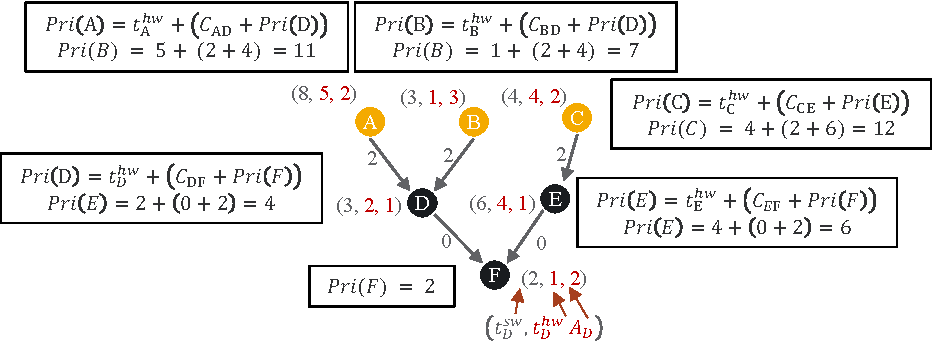
\includegraphics[width=1.0\linewidth]{Figures/methods/static_priorities.pdf}
\caption{\sid{placeholder} Example of bottom-up static-priority computation.}
\label{fig:staticpriorities}
\end{figure}

\paragraph{\textbf{Makespan computation.}}
Given a discrete placement $\hat{\vp}$, we run list scheduling twice, once with software order $\pi_{\mathrm{learn}}^{sw}$ and once with $\pi_{\mathrm{static}}^{sw}$. Let $k \in \{\mathrm{learn},\mathrm{static}\}$ denote the chosen software-order policy. At each scheduling event $t$, the next software task is selected from the ready software set
\begin{equation}
\mathcal{R}_{sw}(t)=\{i\mid \hat{p}_i=0,\ \Pred(i)\subseteq \mathcal{C}(t)\},
\qquad
i_t^{(k)}=\arg\max_{i\in\mathcal{R}_{sw}(t)} \pi_k^{sw}(i),
\end{equation}
with deterministic tie-breaking. Dependency readiness is
\begin{equation}
r_i^{(k)}=\max_{j\in\Pred(i)}\big(f_j^{(k)}+c_{ji}(\hat{\vp})\big),
\end{equation}
and start/finish times are
\begin{equation}
s_i^{(k)}=\max\!\big(r_i^{(k)},t_{i,\mathrm{avail}}^{(k)}\big),
\qquad
f_i^{(k)}=s_i^{(k)}+t_i(\hat{\vp}),
\end{equation}
where
\begin{equation}
t_{i,\mathrm{avail}}^{(k)}=
\begin{cases}
t_{SW,\mathrm{avail}}^{(k)}, & \hat{p}_i=0,\\
0, & \hat{p}_i=1,
\end{cases}
\end{equation}
and $t_{SW,\mathrm{avail}}^{(k)}$ is the current availability time of the single software lane, updated after each scheduled software task.

This yields two candidate makespans,
\begin{equation}
T^{\mathrm{learn}}=\max_i f_i^{(\mathrm{learn})},
\qquad
T^{\mathrm{static}}=\max_i f_i^{(\mathrm{static})}.
\end{equation}
For \diffgnn, we define the discrete evaluation score of placement $\hat{\vp}$ as
\begin{equation}
T^\star(\hat{\vp})
=
\min\!\big(T^{\mathrm{learn}},\,T^{\mathrm{static}}\big),
\label{eq:best_of_two_orders}
\end{equation}
and denote the corresponding selected software order by $\hat{\pi}^{sw}$.

\paragraph{\textbf{Optional local refinement.}}
Starting from the repaired placement, we optionally apply local search to explore local changes, such as flipping assignments of critical nodes. Each proposed move is evaluated using the discrete makespan score $T^\star(\hat{\vp})$, and a move is accepted only if it improves the current solution under this evaluation.

\paragraph{\textbf{Final selection.}}
Across all decoded candidates and their refined versions, we select the solution with the smallest final discrete makespan:
\begin{equation}
(\vp^\star,\pi^{sw,\star})
=
\arg\min_{(\hat{\vp},\hat{\pi}^{sw})\in\mathcal{C}}
M(\hat{\vp},\hat{\pi}^{sw}),
\end{equation}
where $\mathcal{C}$ denotes the set of all feasible decoded or refined placements together with their selected software orders. Equivalently, the final makespan reported for \diffgnn is the minimum value of $T^\star(\hat{\vp})$ over all candidates.

For competing algorithms, we use only the LS-based static-priority order, so that all baselines are evaluated under the same standard discrete scheduling rule.




\subsection{Pseudocode of \diffgnn}
Algorithms~\ref{alg:diffgnn_training} and~\ref{alg:diffgnn_inference} summarize the training and discrete inference procedures of \diffgnn.

\begin{algorithm}[!htbp]
\caption{Training of \diffgnn}
\label{alg:diffgnn_training}
\KwIn{Task graph $\gG=(\gV,\gE)$, epochs $T$, area budget $A_{\max}$}
\KwIn{Loss weights $\lambda_e,\lambda_c,\lambda_a,\lambda_b,\lambda_p$}
\KwIn{Temperatures $\tau_o,\tau_r$ and smooth-max parameter $\beta$}
Initialize model parameters $\theta$\;
Construct node and edge features $\mF,\mE$\;

\For{$t=1,\dots,T$}{
    Predict $\tilde{\vp},\tilde{\vpi}^{sw}\gets \mathrm{GNN}_{\theta}(\gG,\mF,\mE)$\;
    
    Build soft precedence from $\tilde{\vpi}^{sw}$ using Sinkhorn relaxation\;
    
    Compute relaxed execution/communication terms $\tilde{t}_i,\tilde{c}_{ji}$\;
    
    Run differentiable scheduler to obtain $\tilde{\vs},\tilde{\vf}$\;
    
    Compute $L_{\mathrm{makespan}},L_{\mathrm{exec}},L_{\mathrm{comm}},L_{\mathrm{area}},L_{\mathrm{reg}}$\;
    
    $L \gets L_{\mathrm{makespan}}
    + \lambda_e L_{\mathrm{exec}}
    + \lambda_c L_{\mathrm{comm}}
    + \lambda_a L_{\mathrm{area}}
    + L_{\mathrm{reg}}$\;
    
    Update $\theta$ via backpropagation\;
}
\end{algorithm}

\begin{algorithm}[!htbp]
\caption{Discrete Inference and Post-Processing}
\label{alg:diffgnn_inference}
\KwIn{Graph $\gG$, trained model, area budget $A_{\max}$, thresholds $\mathcal{T}$}
\KwOut{Best discrete placement $\vp^\star$, software order $\pi^{sw,\star}$, makespan $M^\star$}

Compute $\tilde{\vp},\tilde{\vpi}^{sw}$\;
Initialize $\vp^\star \gets \emptyset$, $\pi^{sw,\star}\gets\emptyset$, $M^\star \gets +\infty$\;

\For{$\tau_d \in \mathcal{T}$}{
    Decode $\hat{\vp}$ by thresholding:
    $\hat{p}_i \gets \mathbb{I}[\tilde{p}_i \ge \tau_d]$\;
    
    Repair $\hat{\vp}$ until $\sum_i \hat{p}_i A_i \le A_{\max}$\;
    
    Refine $\hat{\vp}$ using local search\tcp*[r]{optional}
    
    Compute learned software order $\pi_{\mathrm{learn}}^{sw}$ by sorting $\tilde{\vpi}^{sw}$\;
    Compute static-priority order $\pi_{\mathrm{static}}^{sw}$ on $\hat{\vp}$\;
    
    $T^{\mathrm{learn}} \gets M(\hat{\vp},\pi_{\mathrm{learn}}^{sw})$,
    $T^{\mathrm{static}} \gets M(\hat{\vp},\pi_{\mathrm{static}}^{sw})$\;
    
    $\hat{\pi}^{sw} \gets
    \arg\min_{\pi \in \{\pi_{\mathrm{learn}}^{sw},\,\pi_{\mathrm{static}}^{sw}\}}
    M(\hat{\vp},\pi)$\;
    
    $T^\star(\hat{\vp}) \gets
    \min\!\big(T^{\mathrm{learn}},\,T^{\mathrm{static}}\big)$\;
    
    \If{$T^\star(\hat{\vp}) < M^\star$}{
        $\vp^\star \gets \hat{\vp}$,\quad
        $\pi^{sw,\star} \gets \hat{\pi}^{sw}$,\quad
        $M^\star \gets T^\star(\hat{\vp})$\;
    }
}
\Return{$(\vp^\star,\pi^{sw,\star},M^\star)$}\;
\end{algorithm}




\subsection{Complexity Analysis}

\paragraph{\textbf{Training Complexity.}}
Let $n=|\gV|$, $m=|\gE|$, hidden size $d$, and $L$ GNN layers. The GNN and prediction heads incur a cost of $O\!\big(L(md + nd^2)\big) + O(nd)$. Applying Sinkhorn normalization to an $n \times n$ matrix costs $O(T_{\mathrm{sink}} n^2)$, where $T_{\mathrm{sink}}$ (typically $10$--$12$) is the number of normalization iterations, and computing rank-based pairwise precedence requires $O(n^2)$. The differentiable scheduler adds $O(m + n^2)$.

Thus, the total time complexity per forward pass is $T_{\text{total}} = O\!\big(L(md + nd^2) + m + T_{\mathrm{sink}} n^2 + n^2\big)$. The space complexity is $S_{\text{total}} = O(Lnd + m + n^2)$, where the $n^2$ term (dense ordering tensors) is the primary scalability bottleneck.


\paragraph{\textbf{Post-processing complexity.}}
For each decoded placement, post-processing requires computing the learned software order, the static-priority order, and evaluating discrete schedules under both. The overall cost per decoded placement is $O(m+n\log n)$. Thus, with $|\mathcal{T}|$ decoding thresholds and $R$ local-refinement evaluations, the total post-processing complexity is $O\!\big((|\mathcal{T}|+R)(m+n\log n)\big)$. In practice, this is much smaller than the training cost.

\paragraph{\textbf{Large-graph approximation.}}
For large-scale graphs, we improve scalability by skipping Sinkhorn normalization and directly using ordering logits for pairwise precedence, while restricting software ordering to the top-$k$ high-confidence nodes per task. This reduces pairwise interactions from $O(n^2)$ to $O(nk)$ with $k \ll n$, yielding $T_{\text{total}} = O\!\big(L(md+nd^2)+m+nk\big)$ and $S_{\text{total}} = O(Lnd+m+nk)$.
\section{Experiments}
In this section, we answer the following questions.
\subsection{Dataset and settings}

\subsection{Makespan comparison}

% random: DAG 32, LSSP 32, SWPRIO -, BEST 32
% greedy: DAG 32, LSSP 32, SWPRIO -, BEST 32
% diff_gnn: DAG 31, LSSP 31, SWPRIO -, BEST 31
% diff_gnn_order: DAG 31, LSSP 31, SWPRIO 29, BEST 29
% gcps: DAG 32, LSSP 32, SWPRIO -, BEST 32
% pso: DAG 83, LSSP 83, SWPRIO -, BEST 83
% dbpso: DAG 29, LSSP 29, SWPRIO -, BEST 29
% clpso: DAG 30, LSSP 30, SWPRIO -, BEST 30
% ccpso: DAG 32, LSSP 32, SWPRIO -, BEST 32
% esa: DAG 30, LSSP 30, SWPRIO -, BEST 30
% shade: DAG 29, LSSP 29, SWPRIO -, BEST 29
% jade: DAG 29, LSSP 29, SWPRIO -, BEST 29
% gl25: DAG 29, LSSP 29, SWPRIO -, BEST 29

\subsection{Ablation Studies}
Base GNN, +sw ordering head, +hw ordering head, +post processing, +greedy fixing, +dag/lssp, +edge weight learning, +features, +objective functions 





\input{7Conclusion}

\clearpage
\bibliographystyle{ACM-Reference-Format}
\bibliography{ReferencesGNN,ReferencesHWSW}

\appendix
\section{Appendix}

\noindent \textbf{Notations:} Table~\ref{tab:Notation} summarizes the main notations used in this paper.

\begin{table}[!htbp]
\caption{Main notations.}
\label{tab:Notation}
\centering
\resizebox{1.0\linewidth}{!}{
\begin{tabular}{l l l}
\toprule
$\gG(\gV,\gE)$ & $\triangleq$ & Task graph \\
$(j,i)$ & $\triangleq$ & Dependency edge $j \rightarrow i$ \\
$t_i^{sw},\,t_i^{hw}$ & $\triangleq$ & SW/HW execution costs \\
$A_i,\,A_{\max}$ & $\triangleq$ & Node area and area budget \\
$C_{ji}$ & $\triangleq$ & Communication cost on $(j,i)$ \\

$\vp,\tilde{\vp},\hat{\vp}$ & $\triangleq$ & Discrete, relaxed, and decoded placements \\
$p_i,\tilde{p}_i,\hat{p}_i$ & $\triangleq$ & Corresponding node assignments \\
$\pi^{sw},\,\tilde{\vpi}^{sw}$ & $\triangleq$ & Discrete and relaxed software order \\
$\pi_{\mathrm{learn}}^{sw},\,\pi_{\mathrm{static}}^{sw}$ & $\triangleq$ & Learned and static software orders \\

$\vs,\vf$ & $\triangleq$ & Discrete start and finish times \\
$\tilde{\vs},\tilde{\vf}$ & $\triangleq$ & Relaxed start and finish times \\
$M(\vp,\pi^{sw})$ & $\triangleq$ & Discrete makespan \\
$\widetilde{M}(\tilde{\vp},\tilde{\vpi}^{sw})$ & $\triangleq$ & Relaxed makespan \\
$\tilde{t}_i(\tilde{\vp}),\,\tilde{c}_{ji}(\tilde{\vp})$ & $\triangleq$ & Relaxed execution and communication \\
$\mathrm{SMax}_{\beta}(\cdot)$ & $\triangleq$ & Smooth maximum \\
\bottomrule
\end{tabular}
}
\end{table}


% \section{Illustrative 6-node example.}
\label{app:illustration}

Let us consider the task graph of Figure~\ref{fig:demosoftmakespan}. The numerical values below are illustrative demo values used only to explain the differentiable soft scheduler.

\begin{figure}[!htbp]
\centering
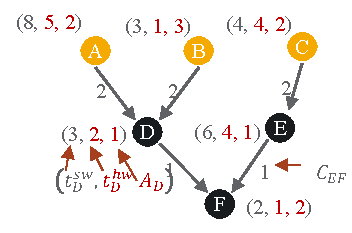
\includegraphics[width=0.52\linewidth]{Figures/methods/demosoftmakespan.pdf}
\caption{Illustrative 6-node fork-join task graph used to explain the differentiable soft scheduler. Each node is annotated with $(t_i^{sw}, t_i^{hw}, A_i)$ and each edge label denotes communication cost.}
\label{fig:demosoftmakespan}
\end{figure}

The graph has dependencies
\[
A \rightarrow D,\quad B \rightarrow D,\quad C \rightarrow E,\quad D \rightarrow F,\quad E \rightarrow F.
\]

For this example, the placement head predicts
\begin{equation}
\tilde{\vp}=[0.05,\,0.05,\,0.05,\,0.95,\,0.95,\,0.95]^\top,
\end{equation}
for tasks $(A,B,C,D,E,F)$, indicating that $A,B,C$ are nearly assigned to software, while $D,E,F$ are nearly assigned to hardware. The ordering head predicts
\begin{equation}
\tilde{\vpi}^{sw}=[0.00,\,-1.00,\,1.00,\,-0.50,\,-0.75,\,-0.25]^\top.
\end{equation}

Using the task costs in Figure~\ref{fig:demosoftmakespan}, the relaxed execution times are
\begin{align}
\tilde t_A &= 0.05\cdot 5 + 0.95\cdot 8 = 7.85, &
\tilde t_B &= 0.05\cdot 1 + 0.95\cdot 3 = 2.90, \\
\tilde t_C &= 0.05\cdot 4 + 0.95\cdot 4 = 4.00, &
\tilde t_D &= 0.95\cdot 2 + 0.05\cdot 3 = 2.05, \\
\tilde t_E &= 0.95\cdot 4 + 0.05\cdot 6 = 4.10, &
\tilde t_F &= 0.95\cdot 1 + 0.05\cdot 2 = 1.05.
\end{align}
Similarly, the soft communication on the cut edges is
\begin{equation}
\tilde c_{AD}=\tilde c_{BD}=\tilde c_{CE}=|0.05-0.95|\cdot 2 = 1.8,
\end{equation}
while $\tilde c_{DF}=\tilde c_{EF}=0$ because the corresponding communication cost is $0$.

\paragraph{\textbf{Step 1: ordering head \(\rightarrow\) Sinkhorn matrix \(\rightarrow\) expected ranks.}}
Using the score-to-position compatibility
\begin{equation}
L_{ai} = -\frac{(\tilde{\pi}_i^{sw}-u_a)^2}{\tau_o},
\qquad
u_a = 1-\frac{2a}{n-1},
\quad a=0,\ldots,n-1,
\end{equation}
Sinkhorn normalization yields the soft permutation matrix
\begingroup
\setlength{\arraycolsep}{3pt}
\begin{equation}
\scriptsize
\mP^{sw}\approx
\begin{bmatrix}
0.181 & 0.002 & 0.695 & 0.029 & 0.008 & 0.084\\
0.332 & 0.015 & 0.257 & 0.120 & 0.047 & 0.229\\
0.271 & 0.060 & 0.043 & 0.218 & 0.128 & 0.280\\
0.143 & 0.155 & 0.005 & 0.255 & 0.224 & 0.219\\
0.056 & 0.302 & 0.000 & 0.223 & 0.291 & 0.128\\
0.017 & 0.467 & 0.000 & 0.155 & 0.302 & 0.060
\end{bmatrix},
\end{equation}
\endgroup
where rows correspond to positions \(a=0,\ldots,5\) and columns correspond to tasks \((A,B,C,D,E,F)\).

The expected ranks are then
\begin{equation}
\tilde r_i=\sum_{a=0}^{n-1} a\,\mP^{sw}_{ai},
\end{equation}
which gives
\begin{equation}
\tilde{\vr}^{sw}\approx
[1.613,\;4.141,\;0.357,\;2.986,\;3.649,\;2.258]^\top.
\end{equation}
Hence the induced global soft order is
\[
C \prec A \prec F \prec D \prec E \prec B,
\]
and the induced software order over the three nearly-software tasks is
\[
C \prec A \prec B.
\]

\paragraph{\textbf{Step 2: expected ranks \(\rightarrow\) before matrix.}}
Using the rank-sigmoid approximation,
\begin{equation}
B^{sw}_{ji}
=
\sigma\!\left(\frac{\tilde r_i-\tilde r_j}{\tau_r}\right),
\qquad
B^{sw}_{ii}=0,
\end{equation}
we obtain the soft before matrix
\begingroup
\setlength{\arraycolsep}{3pt}
\begin{equation}
\scriptsize
\mB^{sw}\approx
\begin{bmatrix}
0     & 0.999 & 0.027 & 0.981 & 0.997 & 0.863\\
0.001 & 0     & 0     & 0.036 & 0.197 & 0.005\\
0.973 & 1.000 & 0     & 0.999 & 1.000 & 0.996\\
0.019 & 0.964 & 0.001 & 0     & 0.869 & 0.111\\
0.003 & 0.803 & 0     & 0.131 & 0     & 0.018\\
0.137 & 0.995 & 0.004 & 0.889 & 0.982 & 0
\end{bmatrix},
\end{equation}
\endgroup
so, for example,
\[
B^{sw}_{CA}=0.973,\qquad B^{sw}_{CB}=1.000,\qquad B^{sw}_{AB}=0.999,
\]
which strongly supports the order \(C \prec A \prec B\).

\paragraph{\textbf{Step 3: gate using placement probabilities.}}
Since ordering matters only when both tasks are likely to execute in software, we use the gate
\begin{equation}
\mG^{sw}=(1-\tilde{\vp})(1-\tilde{\vp})^\top
=
\begin{bmatrix}
0.9025\,\mathbf{1}_{3\times 3} & 0.0475\,\mathbf{1}_{3\times 3}\\
0.0475\,\mathbf{1}_{3\times 3} & 0.0025\,\mathbf{1}_{3\times 3}
\end{bmatrix},
\end{equation}
because \(1-\tilde p_i=0.95\) for \(A,B,C\) and \(1-\tilde p_i=0.05\) for \(D,E,F\).

The effective resource-order matrix is
\begin{equation}
\mR^{sw}=\mB^{sw}\odot \mG^{sw},
\end{equation}
which gives
\begingroup
\setlength{\arraycolsep}{3pt}
\begin{equation}
\scriptsize
\mR^{sw}\approx
\begin{bmatrix}
0     & 0.902 & 0.024 & 0.047 & 0.047 & 0.041\\
0.001 & 0     & 0     & 0.002 & 0.009 & 0    \\
0.878 & 0.902 & 0     & 0.047 & 0.047 & 0.047\\
0.001 & 0.046 & 0     & 0     & 0.002 & 0    \\
0     & 0.038 & 0     & 0     & 0     & 0    \\
0.006 & 0.047 & 0     & 0.002 & 0.002 & 0
\end{bmatrix}.
\end{equation}
\endgroup
In particular,
\[
R^{sw}_{AB}=0.902,\qquad
R^{sw}_{CA}=0.878,\qquad
R^{sw}_{CB}=0.902,
\]
which strongly prefers \(C\) before \(A\) and \(B\), and \(A\) before \(B\).

\paragraph{\textbf{Step 4: DAG readiness and software readiness.}}
To make the effect concrete, we use the hard-order interpretation induced by the soft ranks. For the nearly-software tasks \(A,B,C\), the DAG-readiness values are
\[
s_A^{dag}=s_B^{dag}=s_C^{dag}=0,
\]
since they are source nodes. Thus, their ordering is driven entirely by the software-readiness term. Under the induced software order \(C\prec A\prec B\), we obtain approximately
\begin{align}
s_C^{sw} &\approx 0, &
\tilde s_C &\approx \max(s_C^{dag},s_C^{sw}) = 0, &
\tilde f_C &\approx 0 + 4.00 = 4.00,\\
s_A^{sw} &\approx \tilde f_C = 4.00, &
\tilde s_A &\approx \max(0,4.00) = 4.00, &
\tilde f_A &\approx 4.00 + 7.85 = 11.85,\\
s_B^{sw} &\approx \tilde f_A = 11.85, &
\tilde s_B &\approx \max(0,11.85) = 11.85, &
\tilde f_B &\approx 11.85 + 2.90 = 14.75.
\end{align}

Now consider the hardware tasks. Since \(D\) depends on both \(A\) and \(B\),
\begin{equation}
s_D^{dag}\approx \max(\tilde f_A+\tilde c_{AD},\,\tilde f_B+\tilde c_{BD})
=
\max(11.85+1.8,\;14.75+1.8)
=
16.55,
\end{equation}
and \(s_D^{sw}\approx 0\), so
\[
\tilde s_D\approx 16.55,\qquad
\tilde f_D\approx 16.55+2.05=18.60.
\]
Similarly, since \(E\) depends on \(C\),
\begin{equation}
s_E^{dag}\approx \tilde f_C+\tilde c_{CE}=4.00+1.8=5.80,
\end{equation}
hence
\[
\tilde s_E\approx 5.80,\qquad
\tilde f_E\approx 5.80+4.10=9.90.
\]
Finally, \(F\) depends on both \(D\) and \(E\), so
\begin{equation}
s_F^{dag}\approx \max(\tilde f_D,\tilde f_E)=\max(18.60,9.90)=18.60,
\end{equation}
which yields
\[
\tilde s_F\approx 18.60,\qquad
\tilde f_F\approx 18.60+1.05=19.65.
\]
Thus, the induced relaxed makespan is approximately
\[
L_{\mathrm{soft\mbox{-}makespan}} \approx 19.65.
\]

\paragraph{\textbf{Why \(C\prec A\prec B\) is better than \(A\prec B\prec C\).}}
If the software order were instead \(A\prec B\prec C\), then the same hard-order approximation gives
\[
\tilde f_A\approx 7.85,\qquad
\tilde f_B\approx 10.75,\qquad
\tilde f_C\approx 14.75.
\]
Therefore,
\[
s_D^{dag}\approx \max(7.85+1.8,\;10.75+1.8)=12.55,
\qquad
\tilde f_D\approx 14.60,
\]
while
\[
s_E^{dag}\approx 14.75+1.8=16.55,
\qquad
\tilde f_E\approx 20.65.
\]
This delays the \(C\rightarrow E\rightarrow F\) branch, and hence
\[
s_F^{dag}\approx \max(14.60,\;20.65)=20.65,
\qquad
\tilde f_F\approx 21.70.
\]
Thus,
\[
\mathrm{makespan}(C\prec A\prec B)\approx 19.65
\;<\;
\mathrm{makespan}(A\prec B\prec C)\approx 21.70.
\]

The reason is that the \(C\rightarrow E\) branch is the slower downstream branch: once \(C\) finishes, task \(E\) still needs about \(4.10\) units to complete, whereas the \(A,B\rightarrow D\) branch needs only about \(2.05\) units after both \(A\) and \(B\) finish. Prioritizing \(C\) earlier therefore reduces the final critical path.

\paragraph{\textbf{Why DAG-only readiness is insufficient.}}
Without the ordering head, a scheduler based only on DAG readiness cannot distinguish among the ready source tasks \(A,B,C\), because all three have
\[
s_A^{dag}=s_B^{dag}=s_C^{dag}=0.
\]
Any topological order, such as \(A\prec B\prec C\) or \(C\prec A\prec B\), is valid from the precedence perspective alone. However, these orders produce different software serialization patterns and different makespans. The ordering head resolves this ambiguity by producing a structured pairwise precedence matrix, which allows the soft scheduler to model resource-induced serialization in addition to DAG constraints.

% \pagebreak
\section{Pseudocode}

\begin{algorithm}[!htbp]
\caption{Training of \diffgnn}
\label{alg:diffgnn_trainingapp}
\KwIn{Task graph $\gG=(\gV,\gE)$, epochs $T$, area budget $A_{\max}$}
\KwIn{Area penalty weight $\lambda_a$, ordering temperature $\tau_o$, smooth-max parameter $\beta$}
Initialize model parameters $\theta$\;

\For{$t=1,\dots,T$}{
    Construct node and edge features $\mF,\mE$\;
    Predict relaxed placement and ordering scores
    $\vp,\vq^{sw} \gets \mathrm{GNN}_{\theta}(\gG,\mF,\mE)$,
    where $\vp\in[0,1]^n$ and $\vq^{sw}\in\mathbb{R}^n$\;

    Convert ordering scores to a soft resource-order matrix\;
    $\mP^{sw}\gets \mathrm{Sinkhorn}(\vq^{sw}/\tau_o)$\;
    $\mB^{sw}\gets \mathrm{BeforeMatrix}(\mP^{sw})$\;
    $\forall (j,i)\in\gV\times\gV:\;
    B^{res}_{j,i}\gets B^{sw}_{j,i}(1-p_j)(1-p_i)$\;

    Compute soft execution and communication costs\;
    $\forall i\in\gV:\;
    \tilde{t}_i \gets p_i t_i^{hw} + (1-p_i)t_i^{sw}$\;
    $\forall (j,i)\in\gE:\;
    \tilde{c}_{ji} \gets |p_j-p_i|\,c_{ji}$\;

    Process nodes in topological order\;
    \ForEach{$i\in\gV$}{
        $R_{\mathrm{dag}}(i)\gets
        \mathrm{SMax}_{\beta}\!\Big(\{0\}\cup\{f_j+\tilde{c}_{ji}: j\in\mathrm{pred}(i)\}\Big)$\;

        $R_{\mathrm{res}}(i)\gets
        \mathrm{SMax}_{\beta}\!\Big(\{0\}\cup\{f_j+\alpha\log(B^{res}_{j,i}+\varepsilon): j\neq i\}\Big)$\;

        $s_i \gets \mathrm{SMax}_{\beta}\!\big(R_{\mathrm{dag}}(i), R_{\mathrm{res}}(i)\big)$\;
        $f_i \gets s_i+\tilde{t}_i$\;
    }

    $L_{\mathrm{soft\mbox{-}makespan}}
    \gets
    \mathrm{SMax}_{\beta}\!\big(\{f_i:i\in\gV_{\mathrm{sink}}\}\big)$\;

    $L_{\mathrm{exec}} \gets \sum_{i\in\gV}\tilde{t}_i$\;
    $L_{\mathrm{comm}} \gets \sum_{(j,i)\in\gE}\tilde{c}_{ji}$\;
    $L_{\mathrm{area}}
    \gets
    \left[\max\!\left(0,\sum_{i\in\gV}p_iA_i-A_{\max}\right)\right]^2$\;

    $L \gets L_{\mathrm{makespan}} + L_{\mathrm{exec}} + L_{\mathrm{comm}} + \lambda_a L_{\mathrm{area}}+ L_\mathrm{reg}$\;

    Update $\theta$ via backpropagation\;
}
\end{algorithm}

\begin{algorithm}[!htbp]
\caption{Decoding and Refinement}
\label{alg:diffgnn_inferenceapp}
\KwIn{Graph $\gG$, trained model, area budget $A_{\max}$, thresholds $\mathcal{T}$}
\KwOut{Best partition $\vx^\star$}

Compute $\vp$, $\vq^{sw}$\;

Initialize $\vx^\star \gets \emptyset$, $M^\star \gets +\infty$\;

\For{$\tau_d \in \mathcal{T}$}{
    Decode $\vx$: $x_i = \mathbb{I}[p_i \ge \tau_d]$\;

    \While{$\sum_i x_i A_i > A_{\max}$}{
        Move a hardware node to software\;
    }

    Refine/improve $\vx$ (local search)\;    
    Compute makespan $M(\vx)$ using LSSP\;

    \If{$M(\vx) < M^\star$}{
        $\vx^\star \gets \vx$, \quad $M^\star \gets M(\vx)$\;
    }
}

\Return{$\vx^\star$}\;
\end{algorithm}


% \newpage\pagebreak

% \begin{figure*}[!t]
% \centering
% \begin{tikzpicture}[
%     font=\small,
%     >=Latex,
%     flow/.style={->, draw=black, line width=0.9pt},
%     line/.style={draw=black, line width=0.8pt},
%     thinann/.style={draw=black, line width=0.45pt},
%     task/.style={circle, draw=black!75, line width=0.7pt, minimum size=4.5mm, inner sep=0pt, fill=white},
%     tuple/.style={font=\scriptsize, text=black!80},
%     edgew/.style={font=\scriptsize, inner sep=1pt, fill=white, text=black!80},
%     gnn/.style={draw=black!75, rounded corners=2.2mm, line width=0.85pt, fill=gray!8,
%                 minimum width=1.95cm, minimum height=0.88cm, align=center, inner sep=3pt},
%     box/.style={draw=black!75, line width=0.85pt, fill=gray!8, inner sep=4pt, align=center},
%     topbrace/.style={decorate, decoration={brace, amplitude=4pt, raise=2pt}, draw=black, line width=0.8pt},
%     stagebox/.style={draw=black!75, rounded corners=2.2mm, line width=0.9pt, inner sep=6pt}
% ]

% % =========================================================
% % Input preparation
% % =========================================================
% \node[task] (A) at (0.90,2.90) {A};
% \node[task] (B) at (1.65,2.90) {B};
% \node[task] (C) at (2.40,2.90) {C};
% \node[task] (D) at (1.18,2.05) {D};
% \node[task] (E) at (2.08,2.05) {E};
% \node[task] (F) at (1.60,1.18) {F};

% % node tuples relative to nodes
% \node[tuple, above=3pt of A] {(8, 5, 2)};
% \node[tuple, above=3pt of B] {(3, 1, 3)};
% \node[tuple, above=3pt of C] {(4, 4, 2)};
% \node[tuple, left=3pt of D] {(3, 2, 1)};
% \node[tuple, right=3pt of E] {(6, 4, 1)};
% \node[tuple, right=4pt of F] {(2, 1, 2)};

% % DAG edges
% \draw[flow] (A) -- node[edgew, pos=0.57, left=0.5pt] {2} (D);
% \draw[flow] (B) -- node[edgew, pos=0.52, right=0.5pt] {2} (D);
% \draw[flow] (C) -- node[edgew, pos=0.55, right=0.5pt] {2} (E);
% \draw[flow] (D) -- (F);
% \draw[flow] (E) -- node[edgew, pos=0.56, right=0.5pt] {1} (F);

% % thin feature pointers
% \node[font=\scriptsize, text=black!80, anchor=west] (dfeat) at (0.10,0.34)
% {$(t_D^{\mathrm{sw}},\,t_D^{\mathrm{hw}},\,A_D)$};
% \draw[thinann] (0.55,0.57) -- (1.00,1.63);
% \draw[thinann] (0.95,0.57) -- (1.15,1.63);
% \draw[thinann] (1.35,0.57) -- (1.29,1.63);

% \node[font=\scriptsize, text=black!80, anchor=west] at (2.68,1.16) {$C_{EF}$};
% \draw[thinann] (2.58,1.16) -- (1.92,1.16);

% % =========================================================
% % Training: GNN + heads + loss
% % =========================================================
% \node[gnn] (gnn) at (4.65,2.05) {$\mathit{GNN}_{\theta}(\gG,\mF,\mE)$};

% % graph -> gnn
% \draw[flow] (2.95,2.05) -- (gnn.west);

% % heads
% \node[box, anchor=west, minimum width=2.10cm, minimum height=0.98cm] (place) at (6.35,2.58)
% {Placement head\\[1pt]$\tilde{\vp}\in[0,1]^n$};

% \node[box, anchor=west, minimum width=2.10cm, minimum height=0.98cm] (order) at (6.35,1.22)
% {Ordering head\\[1pt]$\tilde{\vpi}^{\mathrm{sw}}\in[-1,1]^n$};

% % gnn -> heads
% \coordinate (split1) at ($(gnn.east)+(0.30,0)$);
% \draw[line] (gnn.east) -- (split1);
% \draw[flow] (split1) |- (place.west);
% \draw[flow] (split1) |- (order.west);

% % loss
% \node[box, anchor=west, text width=3.20cm, font=\scriptsize] (loss) at (9.60,2.00)
% {%
% $L \leftarrow L_{\mathrm{makespan}}(\tilde{\vp},\tilde{\vpi}^{\mathrm{sw}})$\\[1pt]
% $+\lambda_e L_{\mathrm{exec}}(\tilde{\vp}) + \lambda_c L_{\mathrm{comm}}(\tilde{\vp})$\\[1pt]
% $+\lambda_a L_{\mathrm{area}}(\tilde{\vp}) + L_{\mathrm{reg}}(\tilde{\vp},\tilde{\vpi}^{\mathrm{sw}})$%
% };

% % heads -> loss
% \coordinate (split2) at ($(loss.west)+(-0.28,0)$);
% \draw[line] (split2) -- (loss.west);
% \draw[flow] (place.east) -- ++(0.20,0) |- (split2);
% \draw[flow] (order.east) -- ++(0.20,0) |- (split2);

% % enclosing training box
% \node[stagebox, fit=(gnn)(place)(order)(loss)] (trainbox) {};

% % =========================================================
% % Inference and post-processing
% % =========================================================
% \node[box, anchor=west, align=left, text width=4.10cm, font=\scriptsize] (refine) at (14.00,2.0)
% {%
% $\bullet$~Placement $\vp \leftarrow (\tilde{\vp}\geq \tau)$\\
% \hspace*{1.2em}$\circ$~repair area if required\\[2pt]
% $\bullet$~SW order\\
% \hspace*{1.2em}$\circ$~learned order $\vpi_{\mathrm{learn}}^{\mathrm{sw}} \leftarrow \tilde{\vpi}^{\mathrm{sw}}$\\
% \hspace*{1.2em}$\circ$~static order $\vpi_{\mathrm{static}}^{\mathrm{sw}} \leftarrow \text{critical path}$\\[2pt]
% $\bullet$~Refine placement $\vp$\\
% \hspace*{1.2em}$\circ$~local search using $\vpi_{\mathrm{learn}}^{\mathrm{sw}}/\vpi_{\mathrm{static}}^{\mathrm{sw}}$\\[2pt]
% $\bullet$~Select best $(\vp,\vpi^{\mathrm{sw}})$%
% };

% % loss -> inference
% \draw[flow] (loss.east) -- (refine.west);

% % =========================================================
% % Top braces
% % =========================================================
% \draw[topbrace] (0.20,4.32) -- (2.55,4.32)
% node[midway, yshift=10pt, font=\small, text=black!80]
% {Input preparation};

% \draw[topbrace] (2.95,4.32) -- (13.15,4.32)
% node[midway, yshift=10pt, font=\small, text=black!80]
% {Training};

% \draw[topbrace] (13.65,4.32) -- (18.85,4.32)
% node[midway, yshift=10pt, font=\small, text=black!80]
% {Inference \& post-processing};

% \path[use as bounding box] (0.00,0.00) rectangle (19.05,4.72);
% \end{tikzpicture}
% \end{figure*}


\end{document}
\endinput
%%
%% End of file `sample-sigconf.tex'.
